\documentclass[preprint,12pt,aps,pra,showkeys,amsmath,amssymb,superscriptaddress,floatfix]{revtex4-2}
\usepackage[T1]{fontenc}
\usepackage[utf8]{inputenc}
\usepackage{amsmath,amssymb,amsthm,mathtools,mathrsfs}
\usepackage{microtype,booktabs,enumitem}
\usepackage{xcolor,tikz,etoolbox}
\usepackage[skins,breakable]{tcolorbox}
\usepackage{needspace}
% Keep diagram geometry independent of REVTeX preprint body spacing.
\AtBeginEnvironment{tikzpicture}{\linespread{1}\selectfont}
\usetikzlibrary{arrows.meta,positioning,calc,fit,decorations.pathreplacing}
\usepackage{graphicx}
\usepackage{hyperref}

\definecolor{MMBlue}{RGB}{0,82,155}
\definecolor{MMOrange}{RGB}{200,80,0}
\tikzset{
 mmnode/.style={draw=MMBlue,rounded corners=2pt,fill=MMBlue!4,align=left,execute at begin node={\raggedright},text width=5cm,font=\fontsize{10}{12}\selectfont,inner sep=6pt},
 mmimport/.style={mmnode,draw=black!65,fill=black!4},
 mmcandidate/.style={mmnode,draw=MMOrange,dashed,fill=MMOrange!5},
 mmrejected/.style={mmnode,draw=black,densely dotted,fill=black!8},
 mmproof/.style={->,thick,MMBlue},
 mmflow/.style={->,semithick,black!70},
 mmrepair/.style={->,dashed,thick,MMOrange},
 mmcandidatearrow/.style={->,dashed,semithick,MMOrange},
 mmnote/.style={font=\scriptsize,fill=white,inner sep=2pt,align=center}}

\usepackage[section]{placeins}
\setlength{\emergencystretch}{3em}
\setlist{itemsep=3pt,topsep=4pt}
\newtheorem{theorem}{Theorem}[section]
\newtheorem{proposition}[theorem]{Proposition}
\newtheorem{lemma}[theorem]{Lemma}
\newtheorem{corollary}[theorem]{Corollary}
\theoremstyle{definition}
\newtheorem{definition}[theorem]{Definition}
\newtheorem{example}[theorem]{Example}
\theoremstyle{remark}
\newtheorem{remark}[theorem]{Remark}
% Avoid isolated statement headings and single-line paragraph fragments.
\BeforeBeginEnvironment{theorem}{\Needspace{6\baselineskip}}
\BeforeBeginEnvironment{definition}{\Needspace{5\baselineskip}}
\BeforeBeginEnvironment{proposition}{\Needspace{5\baselineskip}}
\BeforeBeginEnvironment{lemma}{\Needspace{5\baselineskip}}
\BeforeBeginEnvironment{corollary}{\Needspace{5\baselineskip}}
\clubpenalty=5000
\widowpenalty=5000
\newcommand{\R}{\mathbb R}\newcommand{\Z}{\mathbb Z}\newcommand{\N}{\mathbb N}
\newcommand{\Pa}{\operatorname{Pa}}\newcommand{\Desc}{\operatorname{Desc}}
\newcommand{\cl}{\operatorname{cl}}\newcommand{\cost}{\operatorname{cost}}
\newcommand{\status}{\operatorname{status}}
% Faculty cards: a visual rail groups the five faculties within one agent.
% The rail has no arrowhead and does not represent a proof dependency.
\newcommand{\mmfacultybadge}[1]{%
 \node[circle,draw=MMBlue,line width=1pt,fill=white,
 minimum size=7mm,inner sep=0pt,font=\sffamily\small\bfseries,text=MMBlue]
 at ([xshift=15pt,yshift=-15pt]frame.north west) {#1};}
\newcommand{\mmfacultyrail}{%
 \draw[MMBlue!80,line width=1pt]
 ([xshift=15pt,yshift=2pt]frame.north west)--
 ([xshift=15pt,yshift=-2pt]frame.south west);}
\newtcolorbox{mmfacultybox}[2]{enhanced,breakable,
 colback=MMBlue!4,colframe=MMBlue!4,boxrule=0pt,arc=3pt,
 left=39pt,right=9pt,top=4pt,bottom=4pt,
 before skip=2pt,after skip=2pt,
 fontupper=\small\linespread{1.1}\selectfont,
 overlay unbroken={\mmfacultyrail\mmfacultybadge{#1}},
 overlay first={\mmfacultyrail\mmfacultybadge{#1}},
 overlay middle={\mmfacultyrail},overlay last={\mmfacultyrail}}
\newcommand{\mmfaculty}[3]{%
 \begin{mmfacultybox}{#1}{#2}
 {\sffamily\bfseries\color{MMBlue}#2}\par\smallskip #3
 \end{mmfacultybox}}
\newcommand{\agent}[9]{%
 \Needspace{8\baselineskip}
 \subsubsection{#1}
 \noindent\textbf{Object.} #2\par
 \noindent\textbf{Role.} #3\par\smallskip
 \mmfaculty{E}{Ego}{#4}
 \mmfaculty{M}{Memory}{#5}
 \mmfaculty{I}{Intellect}{#6}
 \mmfaculty{S}{Sense}{#7}
 \mmfaculty{A}{Action}{#8}
 \smallskip\noindent #9\par}

\usepackage{longtable,array,calc}
\providecommand{\tightlist}{\setlength{\itemsep}{2pt}\setlength{\parskip}{0pt}}
\makeatletter
\def\frontmatter@abstract@produce{\par\addvspace{\frontmatter@preabstractspace}%
\begingroup\prep@absbox\unvbox\absbox\post@absbox\endgroup
\addvspace{\frontmatter@postabstractspace}}
\makeatother
\newcommand{\field}[2]{\par\smallskip\noindent\textbf{#1.} #2\par}
\setlength{\emergencystretch}{5em}
\AtBeginEnvironment{verbatim}{\small\linespread{1.0}\selectfont}


\hypersetup{colorlinks=true,linkcolor=MMBlue,urlcolor=MMBlue,pdfauthor={Dibakar Sigdel}}

\begin{document}

\title{Heine--Borel Theorem\\[4pt]\large An End-to-End Meta-Math Walkthrough}

\author{Dibakar Sigdel}

\affiliation{Mindverse Computing LLC, Lynnwood, WA 98087, USA}

\date{October 2026}

\begin{abstract}

A complete authored walkthrough of heine--borel theorem, with explicit
mathematical contracts, local verification gates, and reusable exports.
The report presents the target theorem, declared imports, a dependency
graph, five-faculty node contracts, a continuous proof, a worked
example, and a hypothesis-repair audit. It is an authored mathematical
exposition, not a deployed-agent transcript or a formal proof-assistant
certificate.

\end{abstract}\maketitle\linespread{1.12}\selectfont

\noindent\textbf{RA-02 / Real Analysis / Report v1}

\section{Target and import contract}

\begin{theorem}

For \(K\subset\mathbb R^n\) with its Euclidean topology, prove that
\(K\) is compact if and only if it is closed and bounded.

\end{theorem}

\subsection{Foundations and permitted imports}

Use completeness of R to prove compactness of closed boxes below, the
Euclidean distance, and finite-volume geometry. Compact means every open
cover has a finite subcover. The proof supplies the needed closed-box
lemma rather than importing Heine--Borel itself.

\clearpage\section{Node interaction workflow}

\begin{center}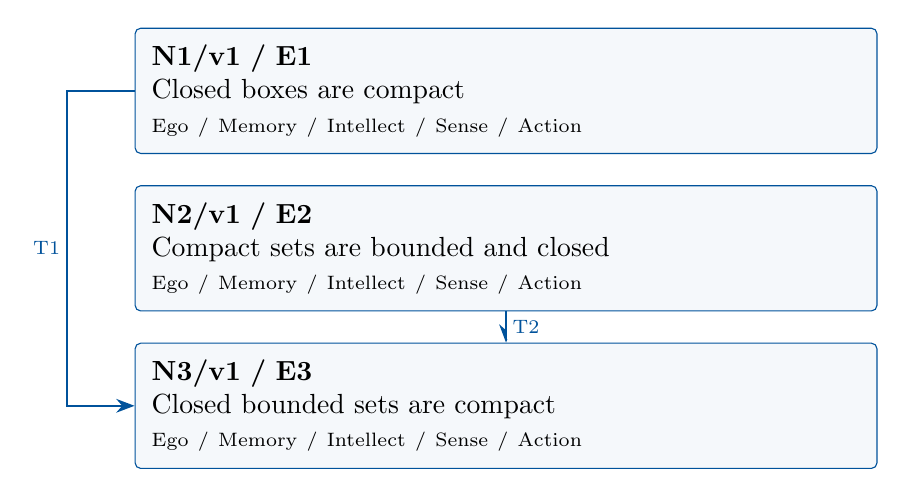
\begin{tikzpicture}[>=Stealth,x=1cm,y=1cm]

\node[mmnode,text width=9cm,minimum height=1.25cm] (N1) at (0,0.0) {\textbf{N1/v1 / E1}\\Closed boxes are compact\\{\scriptsize Ego / Memory / Intellect / Sense / Action}};

\node[mmnode,text width=9cm,minimum height=1.25cm] (N2) at (0,-2.0) {\textbf{N2/v1 / E2}\\Compact sets are bounded and closed\\{\scriptsize Ego / Memory / Intellect / Sense / Action}};

\node[mmnode,text width=9cm,minimum height=1.25cm] (N3) at (0,-4.0) {\textbf{N3/v1 / E3}\\Closed bounded sets are compact\\{\scriptsize Ego / Memory / Intellect / Sense / Action}};

\draw[mmproof] (N1.west) -- (-5.58,0) -- node[mmnote,left] {T1} (-5.58,-4) -- (N3.west);

\draw[mmproof] (N2.south) -- node[mmnote,right] {T2} (N3.north);

\end{tikzpicture}\end{center}

Each box is one mathematical agent containing all five faculties. Blue
arrows carry the versioned exports listed below. The layout gives a
reading order; only drawn arrows assert dependencies. Diagnostic repair
is separate from the proof DAG.

\subsection{Versioned evidence-transfer ledger}

\begingroup\small\linespread{1.05}\selectfont

\Needspace{5\baselineskip}\field{T1: N1/E1/v1 to N3}{Every closed bounded box is compact.}

\field{Receiving activity}{N3: Closed bounded sets are compact}

\field{Compatibility}{Use the same mathematical objects and hypotheses as the source export.
Receiving contract: Closed bounded K; compact box; prior exports E1/v1,
E2/v1}

\Needspace{5\baselineskip}\field{T2: N2/E2/v1 to N3}{Compact K is closed and bounded.}

\field{Receiving activity}{N3: Closed bounded sets are compact}

\field{Compatibility}{Use the same mathematical objects and hypotheses as the source export.
Receiving contract: Closed bounded K; compact box; prior exports E1/v1,
E2/v1}

\endgroup

\clearpage\section{Agent roles and five-faculty activities}\begingroup\small\linespread{1.05}\selectfont\setlist{itemsep=1pt,topsep=2pt}

\subsection{N1/v1: Closed boxes are compact}

\field{Object and role}{Use nested bisection and completeness.}

\field{Inputs}{An open cover of a closed box in \(R^{n}\); foundational imports stated
in §1}

\mmfaculty{E}{Ego}{Own E1/v1: Every closed bounded box is compact.}

\mmfaculty{M}{Memory}{Retain An open cover of a closed box in \(R^{n}\); foundational imports
stated in §1; keep their assumptions and versions attached.}

\mmfaculty{I}{Intellect}{Use nested bisection and completeness.}

\mmfaculty{S}{Sense}{The cover sets are open in an ambient neighborhood; nested endpoints
must be retained.}

\mmfaculty{A}{Action}{Carry out the numbered deductions and publish E1/v1 together with its
hypotheses and proof location.}

\smallskip\noindent\textbf{Numbered mathematical activities}

\begin{enumerate}[label=N1.\arabic*,leftmargin=3.4em]

\item Suppose a box Q has an open cover with no finite subcover.

\item Bisect each side; at least one of the \(2^{n}\) closed subboxes has no
finite subcover, since otherwise their finite covers unite.

\item Continue to nested boxes \(Q_j\) whose diameters tend to 0.

\item Completeness in each coordinate supplies a common point x; it is unique
by the diameter bound.

\item A covering open set contains a ball \(B(x,\varepsilon )\).

\item For large j every point of \(Q_j\) is within its diameter of x, so
\(Q_j\) lies in that one set, contradiction.

\item Degenerate sides cause no difficulty.

\end{enumerate}

\field{Export E1/v1}{Every closed bounded box is compact.}

\field{Acceptance gate}{The cover sets are open in an ambient neighborhood; nested endpoints
must be retained. Publish only after checking every displayed deduction.}

\field{Targeted repair}{If the check fails, revise N1: The cover sets are open in an ambient
neighborhood; nested endpoints must be retained. Recheck dependent nodes
N3.}

\clearpage

\subsection{N2/v1: Compact sets are bounded and closed}

\field{Object and role}{Use a ball cover and point separation.}

\field{Inputs}{Compact K and Euclidean Hausdorff geometry; foundational imports stated
in §1}

\mmfaculty{E}{Ego}{Own E2/v1: Compact K is closed and bounded.}

\mmfaculty{M}{Memory}{Retain Compact K and Euclidean Hausdorff geometry; foundational imports
stated in §1; keep their assumptions and versions attached.}

\mmfaculty{I}{Intellect}{Use a ball cover and point separation.}

\mmfaculty{S}{Sense}{Boundedness alone does not supply a finite subcover.}

\mmfaculty{A}{Action}{Carry out the numbered deductions and publish E2/v1 together with its
hypotheses and proof location.}

\smallskip\noindent\textbf{Numbered mathematical activities}

\begin{enumerate}[label=N2.\arabic*,leftmargin=3.4em]

\item The increasing balls \(B(0,j)\), \(j\ge 1\), cover K; a finite subcover
places it in one sufficiently large ball.

\item For \(x\notin K\) and each \(y\in K\) choose disjoint balls \(U_y\)
around y and \(V_y\) around x, using distance \((x,y)>0\).

\item Finitely many \(U_y\) cover K.

\item The intersection of the corresponding \(V_y\) is an open neighborhood of
x disjoint from K.

\item Thus the complement of K is open and K is closed.

\item The empty set satisfies both conclusions directly.

\end{enumerate}

\field{Export E2/v1}{Compact K is closed and bounded.}

\field{Acceptance gate}{Boundedness alone does not supply a finite subcover. Publish only after
checking every displayed deduction.}

\field{Targeted repair}{If the check fails, revise N2: Boundedness alone does not supply a
finite subcover. Recheck dependent nodes N3.}

\clearpage

\subsection{N3/v1: Closed bounded sets are compact}

\field{Object and role}{Adjoin the complement to an open cover.}

\field{Inputs}{Closed bounded K; compact box; prior exports E1/v1, E2/v1}

\mmfaculty{E}{Ego}{Own E3/v1: \(K\subset R^{n}\) is compact iff closed and bounded.}

\mmfaculty{M}{Memory}{Retain Closed bounded K; compact box; prior exports E1/v1, E2/v1; keep
their assumptions and versions attached.}

\mmfaculty{I}{Intellect}{Adjoin the complement to an open cover.}

\mmfaculty{S}{Sense}{Relative open sets must be converted correctly to a cover of Q.}

\mmfaculty{A}{Action}{Carry out the numbered deductions and publish E3/v1 together with its
hypotheses and proof location.}

\smallskip\noindent\textbf{Numbered mathematical activities}

\begin{enumerate}[label=N3.\arabic*,leftmargin=3.4em]

\item Place K in a closed box Q.

\item Given a relative open cover of K, represent its members as \(K\cap O_i\)
with ambient \(O_i\) open.

\item The \(O_i\) together with \(R^{n}\setminus K\) cover Q.

\item Compactness of Q yields finitely many sets; discarding the complement
leaves finitely many \(O_i\) covering K.

\item This proves compactness and joins both directions of the equivalence.

\end{enumerate}

\field{Export E3/v1}{\(K\subset R^{n}\) is compact iff closed and bounded.}

\field{Acceptance gate}{Relative open sets must be converted correctly to a cover of Q. Publish
only after checking every displayed deduction.}

\field{Targeted repair}{If the check fails, revise N3: Relative open sets must be converted
correctly to a cover of Q. Withhold this terminal result until its gate
passes.}

\endgroup\clearpage\section{Continuous mathematical proof}\label{sec:proof}

Read these steps in order as one proof; the diagram is optional.
Numbered activities identify the specific constructions and deductions
owned by each node.

\subsection{§4.N1 --- Closed boxes are
compact}\label{n1-closed-boxes-are-compact}

\begin{enumerate}
\def\labelenumi{\arabic{enumi}.}
\item
  Suppose a box Q has an open cover with no finite subcover.
\item
  Bisect each side; at least one of the \(2^{n}\) closed subboxes has no
  finite subcover, since otherwise their finite covers unite.
\item
  Continue to nested boxes \(Q_j\) whose diameters tend to 0.
\item
  Completeness in each coordinate supplies a common point x; it is
  unique by the diameter bound.
\item
  A covering open set contains a ball \(B(x,\varepsilon )\).
\item
  For large j every point of \(Q_j\) is within its diameter of x, so
  \(Q_j\) lies in that one set, contradiction.
\item
  Degenerate sides cause no difficulty.
\end{enumerate}

\subsection{§4.N2 --- Compact sets are bounded and
closed}\label{n2-compact-sets-are-bounded-and-closed}

\begin{enumerate}
\def\labelenumi{\arabic{enumi}.}
\item
  The increasing balls \(B(0,j)\), \(j\ge 1\), cover K; a finite
  subcover places it in one sufficiently large ball.
\item
  For \(x\notin K\) and each \(y\in K\) choose disjoint balls \(U_y\)
  around y and \(V_y\) around x, using distance \((x,y)>0\).
\item
  Finitely many \(U_y\) cover K.
\item
  The intersection of the corresponding \(V_y\) is an open neighborhood
  of x disjoint from K.
\item
  Thus the complement of K is open and K is closed.
\item
  The empty set satisfies both conclusions directly.
\end{enumerate}

\subsection{§4.N3 --- Closed bounded sets are
compact}\label{n3-closed-bounded-sets-are-compact}

\begin{enumerate}
\def\labelenumi{\arabic{enumi}.}
\item
  Place K in a closed box Q.
\item
  Given a relative open cover of K, represent its members as
  \(K\cap O_i\) with ambient \(O_i\) open.
\item
  The \(O_i\) together with \(R^{n}\setminus K\) cover Q.
\item
  Compactness of Q yields finitely many sets; discarding the complement
  leaves finitely many \(O_i\) covering K.
\item
  This proves compactness and joins both directions of the equivalence.
\end{enumerate}

\hfill$\square$

\section{Worked orchestration}

For \(K=[0,1]^{2}\), the nested-box proof applies to every open cover,
not just a grid. In contrast (0,1) is covered by set \(s(1/j,1),j\ge 2\)
with no finite subcover; it is bounded but not closed in R.

\subsection{Boundary and hypothesis audit}

The unit coordinate vectors \(e_j\) in the closed unit ball of
\(\ell ^{2}\) have mutual distance \(\sqrt{2}\), so there is no
convergent subsequence. The infinite-dimensional analogue of the box
argument has no \(finite2^{n}\) subdivision and fails. Sense preserves
the finite-dimensional Euclidean scope.

\section{Illustrative failure and repair}

The following is an authored diagnostic scenario. Changed assumptions
define a new contract; they do not retroactively prove the original
statement.

\subsection{Failure and correction}
This is an authored teaching trace, not a recorded agent run.

\begin{enumerate}
\def\labelenumi{\arabic{enumi}.}
\tightlist
\item
  \textbf{Ego \(\to\) Memory:} register the §1 theorem, imports, and
  requested exports before beginning the proof.
\item
  \textbf{Intellect \(\to\) Action:} choose the bridges in §3 and carry
  out the numbered activities in §4; transmit only established E-exports
  along the §2 DAG.
\item
  \textbf{Sense \(\to\) responsible node:} test the specific
  boundary/failure in §5 and the node's individual audit. A failing
  candidate is withheld; downstream nodes may not use it.
\item
  \textbf{Memory + Intellect:} identify whether the error is an omitted
  condition, an invalid inference, or an attempted extension beyond the
  theorem. Restore the exact contract or explicitly state a different
  one.
\item
  \textbf{Action:} redo the affected mathematical activity using the
  repaired condition or inference. Recheck consuming nodes, rather than
  feeding their conclusions back as premises.
\item
  \textbf{Ego:} publish only the supported export with its assumptions
  and proof location. A hypothetical revised export is v2; the written
  proof here is the v1 exposition, not a claim that this repair was
  executed.
\end{enumerate}

\subsection{Hypothesis boundary}
The unit coordinate vectors \(e_j\) in the closed unit ball of
\(\ell ^{2}\) have mutual distance \(\sqrt{2}\), so there is no
convergent subsequence. The infinite-dimensional analogue of the box
argument has no \(finite2^{n}\) subdivision and fails. Sense preserves
the finite-dimensional Euclidean scope.

\subsection{Version and recheck}
Treat any changed assumption as a new contract. Recheck the revised
export and all of its descendants. A backward diagnostic never
establishes an earlier theorem. This is an authored teaching trace, not
an execution log.

\par\medskip\begingroup\small\linespread{1.0}\selectfont\noindent\textbf{Provenance.} This authored proof is complete relative to its declared imports. Reuse
each export with its assumptions, proof, and version. The original
Markdown remains available for comparison.
\par\endgroup

\end{document}
